\section{Comparative Analysis} \label{sec:analysis}

\subsection{Requirements Completeness}

To define the required provenance needed for the ADF in Section 4,  we analyze a healthcare-based ADF use-case (please refer Figure \ref{fig:usecase2})  in which:
\begin{itemize}
\item Data from clinical trials are generated at several participating centres data environment.
\item The data are uploaded electronically by the participating centres to a company called Medidata which offers an electronic data capture and management system for the pharmaceutical industry. 
\item PharComp, a European pharmaceutical business, extracts and downloads the clinical trial data from the Medidata database onto PharComp systems for analysis. 
\item PharComp share data with researchers, for researching on public health. 
\item Researchers publish their analysis in journal articles in the public domain. These data will not include information that identifies the patients, and additional steps are taken to safeguard the patients’ confidentiality.
\item  Explicit consent has been given by trial participants for secondary research use of anonymised data.
\end{itemize}
%The set of actions that has already occurred is retrospective provenance, and is shown in Figure 1 (using the W3C PROV standard [17e]).
%Because the data from EU citizens (amongst others) are being processed, the processing falls within the jurisdiction of GDPR and so that processing must either comply with the principles of GDPR and/or the data must be processed in a fashion which renders them anonymous information. 
%This creates both allowed (prescriptive) and not-allowed (proscriptive) actions.   is prescriptive provenance, and is shown in Figure 3.The proscriptive provenance is shown in Figure 2; the prescriptive provenance is shown in Figure 3.
%In our scenario, a research lab wishes to use PharComp’s anonymized data for further analysis and to publish a report in the public domain.  How does PharComp react to this new situation? This request by the research lab is prospective  provenance related to this action. Figure 4Figure 4 shows this provenance. % 
%Using this information, PharComp must be able to compare the desired actions, i.e., sharing a redacted version to the Research Lab, to defined “allowed” and “not allowed” actions. 




We use this Use Case to confirm that the requirements identified in Section \ref{sec:usecase} are correct (they are also seen in this healthcare use case) and complete (there are no additional requirements identified in the healthcare use case.

The \textbf{Data environment construct} is required to express the data situation within the environments of collection centers, Medidata, PharComp, research labs and open environment. As the data collection centers and research labs  contains sub-environments for various type of data collection and research protocol requirements, confirming the \textbf{“data environments within data environments”} requirement. In the use case, the Medidata and PharComp are type of private data environments and can be accessible to only authorized users and researchers. To express this type of and restriction to these data environments we need to \textbf{represent data, agents and processes}.  

Like the GOND-NRDS use case requirements, in this use case we need to \textbf{annotate the relationship constructs} between the data environments of collection centers and Medidata, where the data is collected and stored instead of data derivation/usage or generation. This will support the semantic meaning of relationship construct in the data provenance. Given the nature of the data collected for the pharmaceutical company, contracts specifying data collection, exchange and control exist (\textbf{contracts}). PharComp has  indirect control over the data release in the open environment in the form of publications and the researcher must follow the code and conduct given by the PharComp, this requirement can be represented with \textbf{access and control} category as mentioned in Table \ref{tab1}. 

Of the requirements presented in Table \ref{tab1} the \textbf{Relationship between data environments} is not not found in this use case, as there are no data environments with multiple institutional ownership and use. However, if the specific example contained an enclave in PharComp in which regulatory employees from a government could review specific data, this requirement would be met. There are no additional requirements that seem necessary to capture the provenance of data situation for ADF.
%\todo{Need a paragraph here, stating either There are No Additional REquirements for DE beyond Table 1. }
\begin{figure}
    \centering
    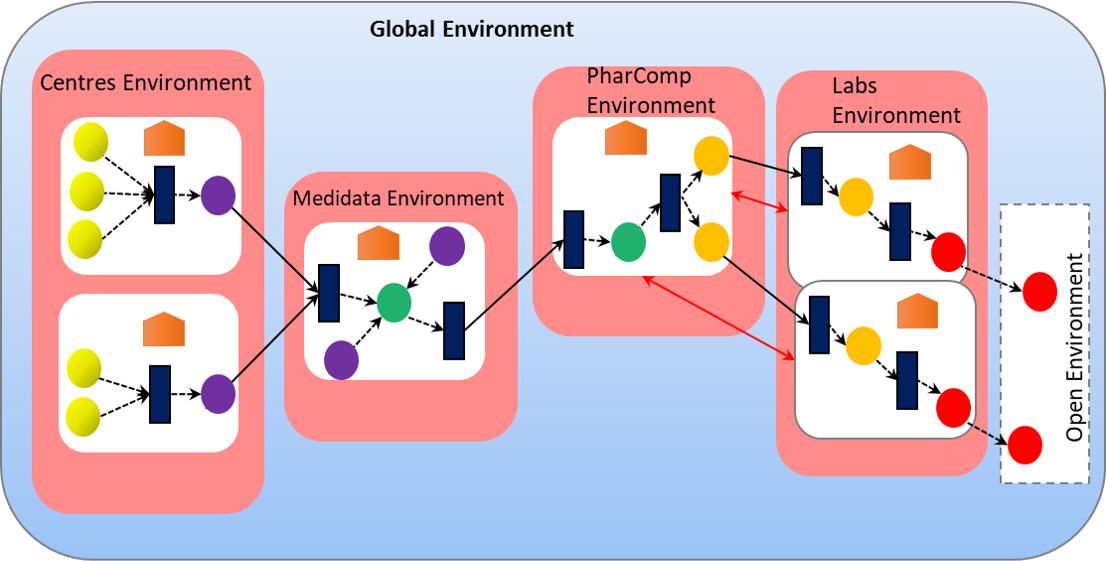
\includegraphics[width=\textwidth]{UseCase2.png}
    \caption{A second ADF Use Case with Data Environments: The red arrows indicate contractual agreements. The black lines indicate data flow. Data environments are indicated by rounded rectangles, A circle represents a piece of data, a rectangle represent a process and a pentagon represents a user in the respective data environment}
    \label{fig:usecase2}
\end{figure}
\subsection{Analysis of Implementation Approaches}
 In Section \ref{sec:usecase} we outlined an ADF Use Case that contains multiple data environments with agents who have a presence in multiple environments, and data that moves between them. Table \ref{tab1} contains the requirements for Data Environments drawn from the GOND-NRDS Use Case and verified by the PharComp Use Case. Table \ref{tab2} shows the data environment representation requirements and the ability of each of the implementation possibilities discussed in Section \ref{sec:impl} to meet those requirements. 

\begin{table}[!htbp]
 \caption{Use case requirements analysis, here Namespace + include attributes and PROV constructs}
  \label{tab2}
  %\centering
  \begin{tabular}{|p{5cm}|c|c|c|c|}
    \hline
    %\cline{2-4}
    \multirow{2}{*}{Representation requirements} &
    \multicolumn{4}{c|}{Support}   
     &  & Bundle & Namespace & Namespace+  &  Bundles+  \\
    \hline
    Data Environment Construct  & \checkmark & \checkmark & \checkmark & \checkmark \\
     \hline
    Data Environments within Data Environments  &  & \checkmark & \checkmark &\checkmark \\
     \hline
    Attaching Attributes to Data Environments &  &  & \checkmark &\checkmark \\
     \hline
     Relationship between Data Environments & \checkmark &  & \checkmark &\checkmark \\
     \hline
     Annotation to   relational constructs  &  &  & \checkmark &\checkmark \\
     
    % \hline
    % Data controller, processor, users and subjects & \checkmark &  & \checkmark &\checkmark \\
     
     
     %\hline
     %Representation of Agents, Data and Processes  & \checkmark & \checkmark  & \checkmark &\checkmark \\
     \hline
     Representation of agents, data and processes within DE  & \checkmark &  \checkmark & \checkmark &\checkmark \\
     \hline
     Contracts  & &  & \checkmark &\checkmark \\
    \hline
     
     Access and control & \checkmark & \checkmark & \checkmark &\checkmark \\
     
    \hline
  \end{tabular}
 
\end{table}

%\todo{The remainder of this until the next sub-section needs a re-write. The namespaces was not represented correctly, so future analysis needs to be smoothed.}
%\todo[color=green!40]{done}

The data environment nesting (i.e. data environments within data  environments) is one of the most important features. For example,  NRDS data environment is the part of University of Barestshire environment. However, with bundles we can not represent  nested data environments because PROV does not allow the nesting of bundles  \cite{moreau2015rationale}. On the other hand the data environments nesting  representation is  supported by Namespaces. For instance, a separate Namespace can be used to indicate a unique data environment.  Thus namespaces+ can also support nesting. This requirement is one of the driving features of bundles+.

The ability to attach attributes to a Data Environment are also one of the most important features of data environments for the ADF to analyse the data situation. Neither bundles or namespaces support attachment of attributes. For example, currently, we cannot express following  using PROV bundle.  \\
 \begin{math}bundle (EX-A:GOND, [prov:envType ="Government", prov:accessType="Restricted") \end{math}. \\
However, the additional structures provided in Namespace+ allows attributes to be maintained with the namespace information. Bundles+ is a much more elegant option, by using the W3C PROVs standard of attaching attributes to other object types, and expanding that notion to bundles+.
 As we have observed in the GOND-NRDS use case (please refer Figure \ref{fig1}), the GOND data environment contains the representation of  collected, processed and shared data along with the data processes, agents, and contracts (i.e. contract with the NRDS), and IT (Information Technology) infrastructure and services. In order to create the provenance graph for GOND data environment representation, the relationship among these elements are supported with PROV properties. For example  \textit{ wasGeneratedBy (entity\_id , activity\_id)}, and \textit{used(activity\_id, entity\_id)} properties are used to represent the relationship between the GOND collected data and process over the data for generating the new dataset for NRDS. Bundles and Namespaces naturally support the representation of agents, processes and entitities using native W3C PROV concepts. On the other hand, supporting additional metadata such as annotation with the relationship constructs is not fully supported in PROV. However, this  can be managed  by attaching additional attributes with the relationship construct as done  in  \cite{pimentel2018versioned} for tracking the changes in entities over the time. We believe that to represent the true meaning of relationship among the data environment elements attaching annotation is necessary. Attaching annotation will also be helpful in selecting an appropriate information disclosure process. %The  data environment as a first class citizen will supports this requirements for GOND-NRDS use case. The GOND-NRDS data, contracts, and data events are supported by Bundles, Namespaces plus, and PROV extension.
 The  PROV extension with extended bundles will supports this requirements for the GOND-NRDS and PharComp use cases. The GOND-NRDS  and PharComp  contracts are  supported by Bundles+  and Namespaces+.
 Moreover, access  control representation requirement is supported by all four constructs.  


%The Bundles construct can be discarded almost immediately. Bundles cannot be nested, and was designed not to support the scoping mechanism of identifiers \cite{moreau2015rationale}. Therefore, the bundle cannot support the requirement of Data Environments in Data %Environments for GOND-NRDS use case. 




     

